%----------------------------------------------------------------------------------------------------
\section{Results}


\begin{figure}
\begin{center}
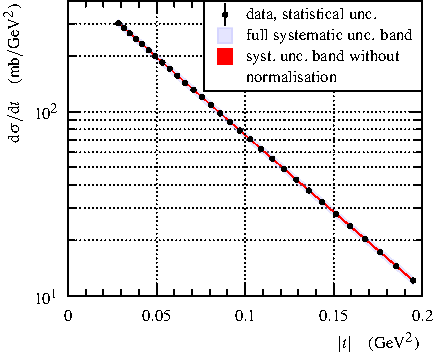
\includegraphics{fig/t_dist.pdf}
\caption{%
\todo{``optimised'' binning}
}
\label{fig:data ob}
\end{center}
\end{figure}

% --- the results drawn from the optimised binning

\todo{add description of fit-quality measures, results in tables}

The final differential cross-section in the ``optimised'' binning is presented in Table~\ref{tab:data}. Since it exhibits an exponential-like fall-off, for visualisation purposes, it is preferable to plot the relative difference of the cross-section from a reference exponential, % subtracting the main component
see Figure~\ref{fig:data rel ob}. This plot immediately suggests a non-exponentiality of the data. To quantify this observation, a series of fits has been made using this parametrisation \todo{comment: physics meaning or simply some math}:
\begin{equation}
\label{fit param}
{\d\sigma\over\d t}(t) = \left. \d\sigma\over\d t\right|_{0} \ \exp\left( \sum\limits_{i = 1}^{N_{b}} b_i\, t^i \right) \:.
\end{equation}
\todo{rephrase} The fits have been performed by minimising the standard $\chi^2$ with the covariance matrix given by the sum of the statistical and systematic components. The fit results are shown in Figure~\ref{fig:data rel ob}, clearly indicating that the purely-exponential fit ($N_b = 1$) is excluded at $7.2\un{\sigma}$ significance. The other two fits present very reasonable p-values and can, therefore, be used for a total cross-section estimation with the optical theorem in the form
\begin{equation}
\label{eq:si tot}
\sigma_{\rm tot}^2 = {16\pi\, (\hbar c)^2\over 1 + \rho^2}\, \left. \d\sigma_{\rm el}\over\d t\right|_0\ ,
\end{equation}
for the first time using a non-exponential extrapolation to $t=0$. Using the COMPETE~\cite{compete} preferred-model extrapolation of $\rho = 0.140\pm 0.007$ yields
\begin{equation}
\label{eq:si tot results}
	\begin{aligned}
		N_b &= 2:\quad \sigma_{\rm tot} = (100.8 \pm 2.1)\un{mb}\ ,\\	% A = 529.3 +- 21.9
		N_b &= 3:\quad \sigma_{\rm tot} = (101.2 \pm 2.1)\un{mb}\ ,\\	% A = 533.5 +- 21.9
	\end{aligned}
\end{equation}
which are well compatible with the previous measurement using the luminosity-independent method~\cite{prl111}.




% --- results from per-mille binning

The incompatibility between a pure exponential behaviour and the data with the ``per-mille'' binning can be shown equally well. However, since the number of points is drastically increased, the $\chi^2$ test does not have sufficient sensitivity, and a different test is used. Assuming that the data can be described by a pure exponential, the fit parameters should have compatible values for fits over different ranges. Such fits are shown in Figure~\ref{fig:data rel cpb0.001}, for regions below and above $|t| = 0.07\un{GeV^2}$. Although the overall fit quality is satisfactory, the difference in fit parameters excludes their compatibility at $7.7\un{\sigma}$. This, in turn, rules out the assumption, the hypothesis of a purely exponential behaviour of the data.
\todo{this test is binning-independent}

\iffalse
	split details
                A = 529.299 +- 21.951
                B1 = -19.678 +- 0.074
                B2 = 514.681 +- 21.953
                B3 = -19.264 +- 0.057

 A1 − A2 = 14.617 ± 1.789 ⇒ 8.2 σ
 B1 − B2 = −0.414 ± 0.056 ⇒ 7.4 σ
\fi




\begin{figure*}
\vskip-5mm
\begin{center}
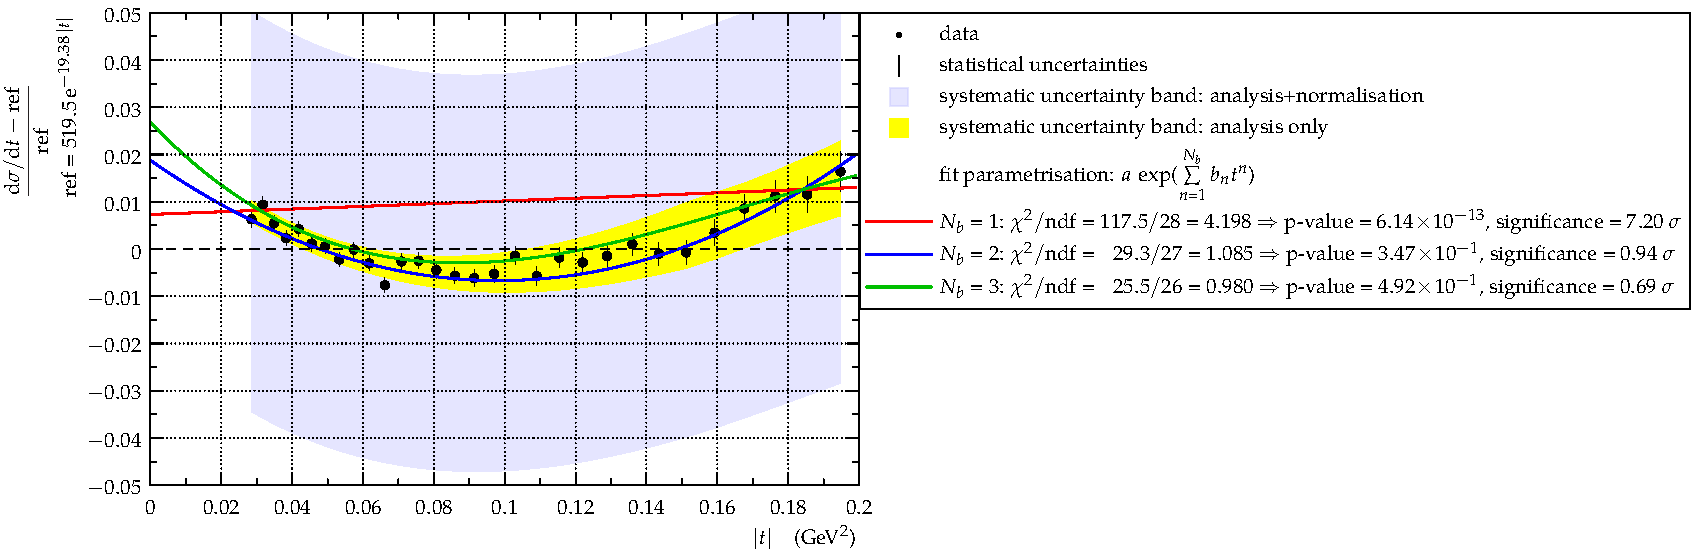
\includegraphics{fig/t_dist_rel_with_fits.pdf}
\vskip-4mm
\caption{%
Differential cross-section using the ``optimised'' binning and plotted as relative difference from a reference exponential (see vertical axis). The black dots represent data points with statistical uncertainty bars. The blue band corresponds to the full systematic uncertainty, the yellow one includes all systematic contributions except the normalisation. The coloured lines correspond to fits with parametrisation Eq.~(\ref{fit param}). The red line lies seemingly too high with respect to the data points, which is a consequence of the systematic degrees of freedom included in the fit.
%
Various fit-quality measures are given in the legend, starting with the $\chi^2$ value after minimisation divided by the number of degrees of freedom (ndf). P-value: probability that a $\chi^2$ value greater than the observed one would be drawn from the $\chi^2$ distribution with the given number of degrees of freedom. Significance: half-width of a central region that needs to be excluded from a normal distribution to get the same integrated probability as the p-value.
}
\label{fig:data rel ob}
\end{center}
\vskip-2mm
\end{figure*}



\begin{figure*}
\begin{center}
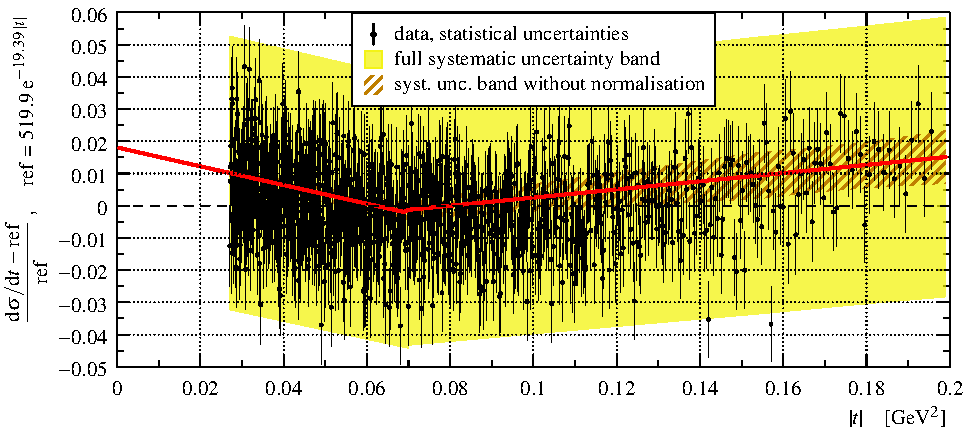
\includegraphics{fig/t_dist_rel_with_split_fit.pdf}
\vskip-4mm
\caption{%
Differential cross-section using the ``per-mille'' binning and plotted as relative difference from the reference exponential (see vertical axis). The black dots represent data points with statistical uncertainty bars. The blue band corresponds to the full systematic uncertainty, the yellow one includes all systematic contributions except the normalisation. The green line shows pure exponential fits in regions below and above $|t| = 0.07\un{GeV^2}$.
}
\label{fig:data rel cpb0.001}
\end{center}
\end{figure*}

